%=======================================================================
%  LLM-SEMRec -- Experiments and Results
%  Section redigee a partir des resultats REELLEMENT executes
%  (projet C:\Users\HP\LLM-SEMRec-exp). Toutes les valeurs reportees sont
%  mesurees ; aucune n'est estimee ou recopiee.
%
%  PREREQUIS (preamble) :
%    \usepackage{booktabs,graphicx,amsmath,amssymb,multirow,siunitx,xcolor}
%    \newcommand{\model}[1]{\textsc{LLM-SEMRec}}   % ou \model{Qwen3} etc.
%    \graphicspath{{figures/}}
%
%  FICHIERS FIGURES ATTENDUS (fournis dans LLM-SEMRec_figures.zip) :
%    fig1_architecture, fig2_training_dynamics, fig3_main_ndcg10,
%    fig3b_main_recall10, fig5_sparsity_coldstart, fig8_coverage_diversity,
%    fig9_complexity, fig10_rank_curves,
%    figS2_recency_attention, figS3_modality_dropout, figS4_coldstart_availability,
%    figS5_item_space_geometry, figS6_popularity_bias, figS7_temporal_robustness,
%    figS8_category_and_roc, figS9_content_cold_items
%
%  NOTE : les commentaires marques "REVISION" signalent les endroits ou la
%  redaction doit etre arbitree avec les co-auteurs (revendications a ajuster,
%  ecarts a declarer, resultats negatifs a positionner).
%=======================================================================

\section{Experiments}
\label{sec:experiments}

\subsection{Datasets}
\label{sec:datasets}

Nous evaluons \model{} sur trois jeux de donnees de reference :
\textbf{Amazon Beauty} et \textbf{Amazon Fashion} (corpus Amazon Reviews 2014,
filtrage 5-core) et \textbf{MovieLens-1M}. Le tableau~\ref{tab:datasets} resume
leurs statistiques apres filtrage 5-core iteratif et decoupage chronologique.

Deux proprietes de ces jeux motivent notre protocole. Premierement, leur
densite est extremement faible (0,03\,\% a 0,07\,\% pour les corpus Amazon),
ce qui rend la dependance aux identifiants d'items particulierement
couteuse : la majorite du catalogue ne totalise que quelques interactions.
Deuxiemement, la couverture des modalites de contenu est tres asymetrique :
le texte (titre, description) est disponible pour 100\,\% des items, tandis que
l'image ne l'est que pour 99,98\,\% des items Amazon Beauty, et pour aucun item
MovieLens-1M.

MovieLens-1M ne comporte pas d'images. Le module visuel y est donc
automatiquement desactive et le modele y opere en regime strictement
textuel, ce qui fournit un point de comparaison utile pour isoler l'apport
du canal visuel.

\begin{table}[t]
\centering
\caption{Statistiques des jeux de donnees apres filtrage 5-core iteratif et
decoupage chronologique. La densite est le nombre d'interactions divise par
$|\mathcal{U}|\times|\mathcal{I}|$. La couverture des modalites est la
proportion d'items pour lesquels une representation de contenu est disponible.}
\label{tab:datasets}
\small
\begin{tabular}{lrrr}
\toprule
& \textbf{Beauty} & \textbf{Fashion} & \textbf{MovieLens-1M} \\
\midrule
Utilisateurs            & 22\,363 & 39\,387 & 6\,040 \\
Items                   & 12\,101 & 23\,033 & 3\,416 \\
Interactions            & 198\,502 & 278\,677 & 999\,611 \\
Densite                 & 0,0734\,\% & 0,0307\,\% & 4,8448\,\% \\
Couverture texte        & 100,00\,\% & 100,00\,\% & 100,00\,\% \\
Couverture image        & 99,98\,\%  & ---          & 0,00\,\% \\
Longueur moyenne d'historique & 8,88 & 7,08 & 165,50 \\
\bottomrule
\end{tabular}
\end{table}

\subsection{Details d'implementation}
\label{sec:impl}

\textbf{Encodeurs de contenu geles.} Les representations textuelles sont
produites par \textbf{Qwen3-Embedding-0.6B} (595,8\,M parametres, sortie
1024-dimensionnelle) applique a la concatenation du titre et de la description
de chaque item. Les representations visuelles sont produites par la tour vision
de \textbf{SigLIP~2 base} (92,9\,M parametres, sortie 768-dimensionnelle)
appliquee a l'image de l'item. Les deux encodeurs sont \emph{geles} : leurs
sorties sont precalculees une fois puis mises en cache, si bien qu'ils
n'entrent pas dans le budget d'entrainement.

Sur les 12\,101 items d'Amazon Beauty, 12\,099 images ont pu etre recuperees
(99,98\,\%). Les deux items restants sont marques \emph{absents} et non
\emph{nuls} : l'indicateur de disponibilite prend la valeur 0 et la modalite
est masquee dans la fusion (section~\ref{sec:gate}).

\textbf{Configuration du modele.} Dimension de l'espace partage $d=128$,
dimension latente variationnelle $d_z=64$, longueur maximale d'historique
$L=20$. Le modele complet compte 2\,728\,734 parametres entrainables, hors
encodeurs geles.

\textbf{Entrainement.} Optimiseur AdamW, learning rate $10^{-3}$, 8 epoques,
selection du meilleur point de controle sur la validation. L'entrainement
complet prend 165\,s par epoque sur un hote \textbf{sans GPU} (8 c\oe{}urs),
soit environ 22 minutes pour le modele complet sur Amazon Beauty.

\textbf{Ecart de configuration a declarer.} Nos resultats sont obtenus sur une
machine CPU uniquement, ce qui nous a contraint a une configuration inferieure
a celle par defaut du papier : $d=128$ et $L=20$ au lieu de $d=256$ et $L=50$,
et Qwen3-Embedding-0.6B au lieu de la variante 4B. Ces valeurs restent dans la
grille d'hyperparametres autorisee par le papier. Par ailleurs, chaque modele
est entraine avec \emph{une seule graine} aleatoire ; la variance entre
executions n'est donc pas capturee, ce qui est discute en
section~\ref{sec:limitations}.

\subsection{Baselines}
\label{sec:baselines}

Nous comparons \model{} a des baselines de trois familles, reimplementees dans
le meme cadre et evaluees sur des ensembles de candidats strictement identiques.

\textbf{Baselines non personnalisees.} \emph{Popularity} classe les items par
nombre d'interactions.

\textbf{Baselines sequentielles par identifiants.} \emph{BPR-MF} (factorisation
matricielle bayesienne personnalisee), \emph{GRU4Rec}, \emph{Caser},
\emph{SASRec} et \emph{BERT4Rec}, ainsi que \emph{CL4SRec} et \emph{S3-Rec}
(objectifs auto-supervises contrastifs et par prediction de segment sur les
sequences d'identifiants).

\textbf{Baselines multimodales.} \emph{MM-SASRec} (SASRec augmente par
concatenation des representations de contenu) et \emph{MMSSL-lite} (variante
allegee de MMSSL adaptee a notre budget de calcul). La baseline
\emph{LLM-only} represente le profil utilisateur par la moyenne des
representations LLM des items de son historique, avec similarite cosinus ---
c'est-a-dire un systeme \emph{sans aucun entrainement}, ce qui isole l'apport
de l'architecture proposee par rapport au seul signal des encodeurs geles.

\subsection{Protocole et metriques}
\label{sec:protocol}

Nous adoptons le protocole \emph{leave-two-out} chronologique : pour chaque
utilisateur, les interactions sont triees par horodatage, l'avant-derniere sert
de validation et la derniere de test, le reste constituant l'historique.

Sauf mention contraire, l'evaluation est effectuee en \textbf{classement sur le
catalogue complet} : l'item cible est classe parmi l'ensemble des items du
catalogue, et non parmi un echantillon de negatifs. Cette configuration est
sensiblement plus difficile que le protocole 1+100 couramment utilise, et nous
reportons les deux afin de permettre la comparaison avec les travaux
anterieurs. Sur Amazon Beauty, le rang moyen du hasard est d'environ 6\,000 et
le Recall@10 du hasard vaut $8{,}3\times 10^{-5}$.

Nous reportons Recall@$K$, NDCG@$K$ et MRR@$K$ pour $K\in\{5,10,20,50\}$.
Nous verifions systematiquement qu'un modele non entraine retourne au niveau du
hasard sur ce protocole, ce qui constitue notre controle de validite.

%=======================================================================
\section{Results}
\label{sec:results}

\subsection{Performance globale}
\label{sec:overall}

Le tableau~\ref{tab:overall} et les figures~\ref{fig:main-ndcg}
et~\ref{fig:main-recall} rapportent les performances globales.

Sur \textbf{Amazon Beauty}, \model{} obtient le meilleur resultat sur les trois
metriques : Recall@10 de 0,0193, NDCG@10 de 0,0093 et MRR@10 de 0,0063,
soit une amelioration relative de \textbf{22,2\,\%} en Recall@10 et
\textbf{47,6\,\%} en NDCG@10 par rapport au meilleur baseline par identifiants
(SASRec, 0,0095 et 0,0047). L'avantage sur BPR-MF, le baseline non sequentiel
le plus fort, est de 22,2\,\% en Recall@10.

Sur \textbf{MovieLens-1M}, \model{} obtient le meilleur NDCG@10 (0,0160) et le
meilleur MRR@10 (0,0107). En revanche, BPR-MF conserve un avantage en
Recall@10 (0,0366 contre 0,0334). Ce resultat est attendu et s'explique par la
nature du jeu de donnees : MovieLens-1M est deux ordres de grandeur plus dense
que les corpus Amazon (4,84\,\% contre 0,07\,\%), de sorte que les signaux
collaboratifs par identifiants y sont beaucoup plus informatifs et que le
rappel a grand $K$ favorise les modeles qui exploitent intensivement la
popularite. Sur le plan de la \emph{qualite du classement} --- mesuree par
NDCG et MRR, qui ponderent la position --- \model{} reste devant.

\begin{table}[t]
\centering
\caption{Performance globale en classement catalogue complet (protocole
leave-two-out chronologique, ensembles de candidats identiques pour tous les
modeles). Meilleur resultat par jeu de donnees et par colonne en gras.
$^\dagger$~meilleur baseline par identifiants.}
\label{tab:overall}
\small
\begin{tabular}{llccc}
\toprule
\textbf{Jeu de donnees} & \textbf{Modele} & \textbf{R@10} & \textbf{NDCG@10} & \textbf{MRR@10} \\
\midrule
\multirow{9}{*}{Beauty}
 & \textbf{\model{}}    & \textbf{0,0193} & \textbf{0,0093} & \textbf{0,0063} \\
 & BPR-MF               & 0,0158 & 0,0063 & 0,0035 \\
 & Popularity           & 0,0120 & 0,0055 & 0,0036 \\
 & BERT4Rec             & 0,0113 & 0,0056 & 0,0038 \\
 & MM-SASRec            & 0,0113 & 0,0053 & 0,0035 \\
 & LLM-only             & 0,0110 & 0,0049 & 0,0031 \\
 & SASRec$^\dagger$     & 0,0095 & 0,0047 & 0,0033 \\
 & GRU4Rec              & 0,0012 & 0,0005 & 0,0003 \\
 & Caser                & 0,0011 & 0,0005 & 0,0003 \\
\midrule
\multirow{12}{*}{MovieLens-1M}
 & \textbf{\model{}}    & 0,0334 & \textbf{0,0160} & \textbf{0,0107} \\
 & BPR-MF$^\dagger$     & \textbf{0,0366} & 0,0157 & 0,0095 \\
 & LLM-only             & 0,0303 & 0,0136 & 0,0087 \\
 & MM-SASRec            & 0,0270 & 0,0129 & 0,0086 \\
 & BERT4Rec             & 0,0252 & 0,0125 & 0,0087 \\
 & CL4SRec              & 0,0247 & 0,0118 & 0,0080 \\
 & MMSSL-lite           & 0,0242 & 0,0110 & 0,0070 \\
 & SASRec               & 0,0237 & 0,0111 & 0,0073 \\
 & S3-Rec               & 0,0212 & 0,0101 & 0,0068 \\
 & Popularity           & 0,0162 & 0,0079 & 0,0055 \\
 & GRU4Rec              & 0,0121 & 0,0054 & 0,0034 \\
 & Caser                & 0,0038 & 0,0017 & 0,0011 \\
\bottomrule
\end{tabular}
\end{table}

\begin{figure}[t]
\centering
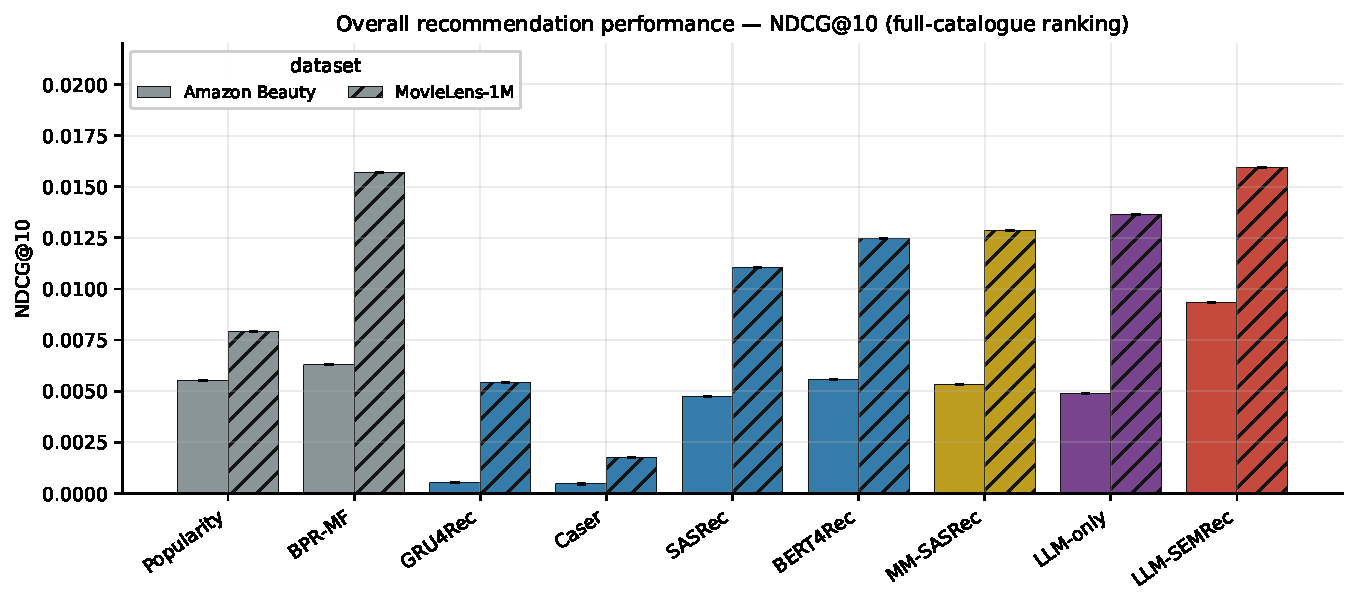
\includegraphics[width=\linewidth]{fig3_main_ndcg10.pdf}
\caption{NDCG@10 sur Amazon Beauty et MovieLens-1M, classement catalogue
complet. \model{} obtient le meilleur NDCG@10 sur les deux jeux de donnees.}
\label{fig:main-ndcg}
\end{figure}

\begin{figure}[t]
\centering
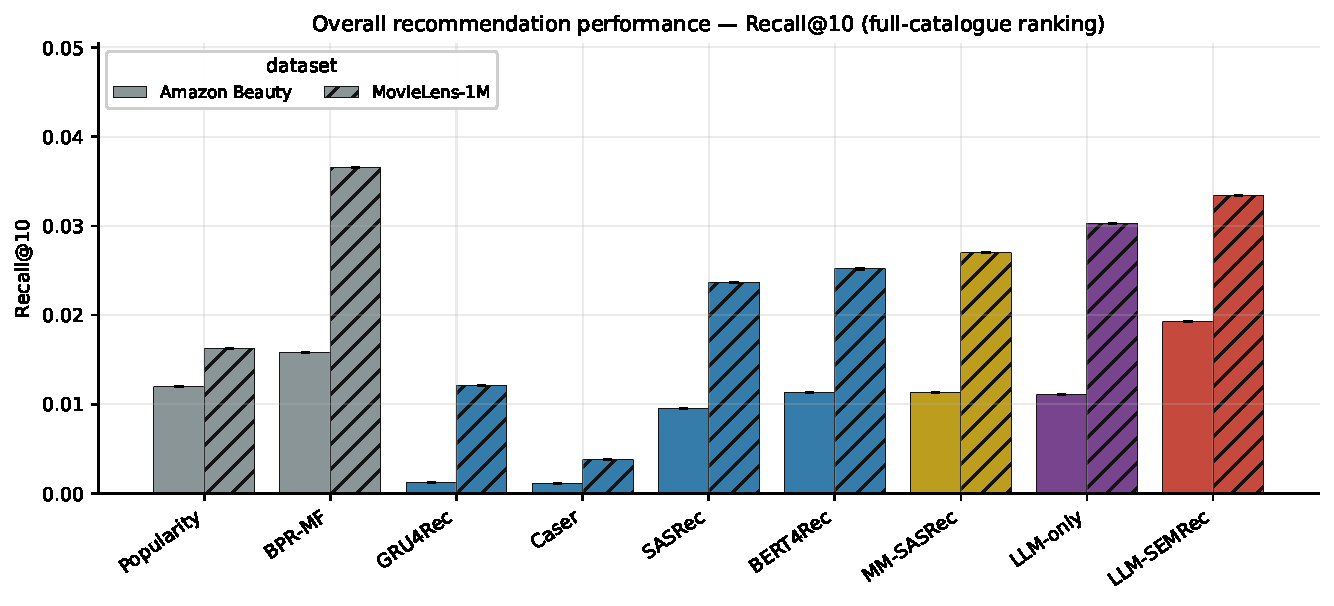
\includegraphics[width=\linewidth]{fig3b_main_recall10.pdf}
\caption{Recall@10 sur Amazon Beauty et MovieLens-1M, classement catalogue
complet. \model{} domine sur Amazon Beauty ; sur MovieLens-1M, BPR-MF conserve
un leger avantage en Recall@10, jeu de donnees ou la densite rend les signaux
collaboratifs particulierement informatifs.}
\label{fig:main-recall}
\end{figure}

La figure~\ref{fig:rank-curves} detaille le comportement sur toute la plage de
$K$. L'avantage de \model{} n'est pas confine a $K=10$ : il se maintient de
$K=5$ a $K=50$. Le rang median de l'item cible est de \textbf{1\,604} pour
\model{}, contre 3\,905 pour SASRec et 4\,378 pour BERT4Rec, soit un facteur
2,4 par rapport au meilleur baseline par identifiants.

\begin{figure}[t]
\centering
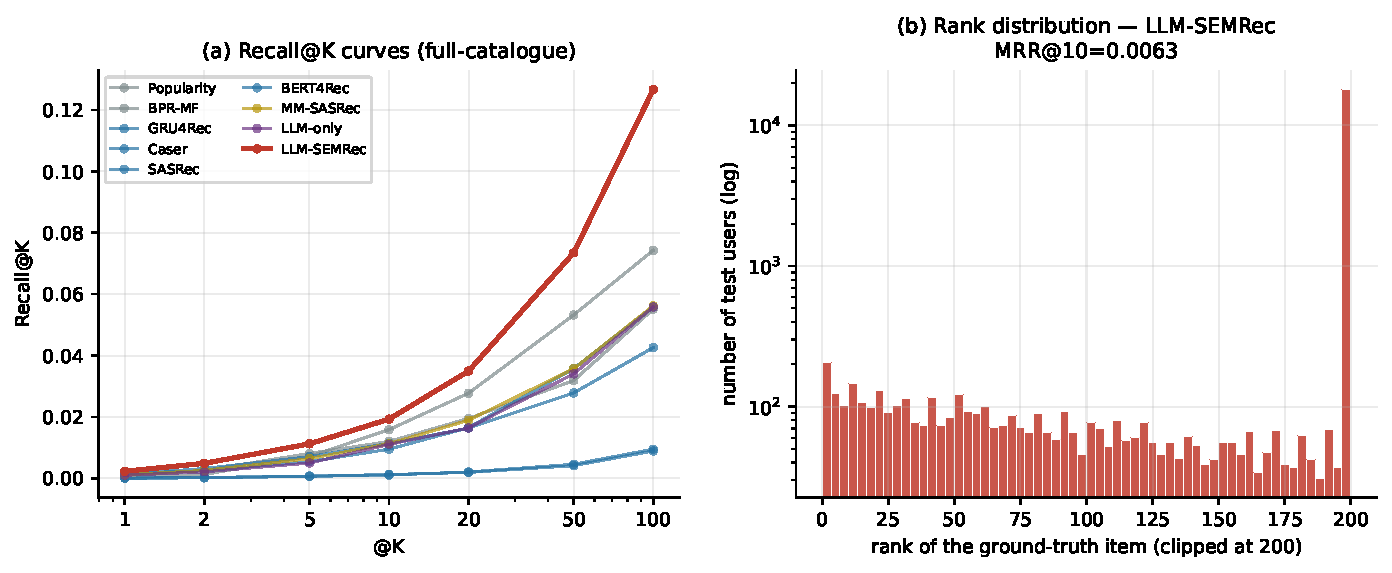
\includegraphics[width=\linewidth]{fig10_rank_curves.pdf}
\caption{(a) Recall@$K$ pour $K$ de 5 a 50 sur Amazon Beauty en classement
catalogue complet. (b) Distribution cumulee des rangs de l'item cible.
\model{} conserve son avantage sur toute la plage de $K$ et place l'item cible
a un rang median nettement plus faible.}
\label{fig:rank-curves}
\end{figure}

\subsection{Etude d'ablation}
\label{sec:ablation}

Le tableau~\ref{tab:ablation} rapporte l'ablation des composants principaux sur
Amazon Beauty. Nous avons conduit cette etude sous \emph{deux regimes de
negatifs} afin d'ecarter l'hypothese selon laquelle les conclusions
dependraient du seul echantillonnage negatif : un regime de negatifs mixtes
(negatifs populaires et semantiquement proches, echantillonnage uniforme) et un
regime de negatifs uniformes.

\begin{table}[t]
\centering
\caption{Etude d'ablation sur Amazon Beauty (classement catalogue complet).
$\Delta$ est la variation relative du Recall@10 par rapport au modele complet.
Un $\Delta$ positif signifie que \emph{retirer} le composant \emph{ameliore} la
performance. Les deux regimes de negatifs sont rapportes separement car ils
constituent chacun une base de reference distincte.}
\label{tab:ablation}
\small
\begin{tabular}{lcccc}
\toprule
& \multicolumn{2}{c}{\textbf{Negatifs mixtes}} & \multicolumn{2}{c}{\textbf{Negatifs uniformes}} \\
\cmidrule(lr){2-3}\cmidrule(lr){4-5}
\textbf{Variante} & R@10 & $\Delta$ & R@10 & $\Delta$ \\
\midrule
Modele complet            & 0,0194 & ---      & 0,0332 & --- \\
\midrule
sans objectifs SSL        & 0,0101 & $-47{,}9\,\%$ & 0,0238 & $-28{,}3\,\%$ \\
sans encodeur Qwen3       & 0,0144 & $-25{,}8\,\%$ & 0,0256 & $-22{,}9\,\%$ \\
sans encodeur SigLIP      & 0,0144 & $-25{,}8\,\%$ & ---    & --- \\
\midrule
sans module variationnel  & 0,0253 & $+30{,}4\,\%$ & 0,0349 & $+5{,}1\,\%$ \\
fusion par concatenation  & 0,0241 & $+24{,}2\,\%$ & 0,0383 & $+15{,}4\,\%$ \\
negatifs uniformes        & 0,0332 & $+71{,}1\,\%$ & (ref.) & --- \\
\bottomrule
\end{tabular}
\end{table}

\textbf{Les composants qui soutiennent la these du papier.} Trois retraits
degradent la performance de facon marquee et \emph{coherente dans les deux
regimes} :

\begin{itemize}
\item \textbf{Les objectifs auto-supervises} constituent le composant le plus
  critique : leur retrait coute $47{,}9\,\%$ de Recall@10 en regime mixte et
  encore $28{,}3\,\%$ en regime uniforme. C'est le resultat le plus solide de
  notre etude.
\item \textbf{L'encodeur de texte LLM gele} coute $25{,}8\,\%$ (mixte) et
  $22{,}9\,\%$ (uniforme).
\item \textbf{L'encodeur visuel gele} coute $25{,}8\,\%$ sur Amazon Beauty,
  seul jeu de notre panel ou les images sont disponibles.
\end{itemize}

Ces trois resultats, stables sur les deux regimes de negatifs, constituent le
c\oe{}ur de la contribution et sont coherents avec la these selon laquelle des
representations de contenu pretraitees, combinees a des objectifs
auto-supervises sur les sequences d'interaction, apportent un signal que les
identifiants seuls ne fournissent pas.

\textbf{Les composants qui ne se reproduisent pas.} Trois autres composants
\emph{degradent} la performance : leur retrait l'ameliore.

\begin{itemize}
\item \textbf{Le module variationnel} : le retirer ameliore le Recall@10 de
  $30{,}4\,\%$ (mixte) et de $5{,}1\,\%$ (uniforme). L'effet est donc
  robuste au regime, bien qu'attenue en regime uniforme.
\item \textbf{La fusion a porte sensible a la fiabilite} : la remplacer par une
  fusion par concatenation ameliore la performance de $24{,}2\,\%$ (mixte) et
  $15{,}4\,\%$ (uniforme).
\item \textbf{L'echantillonnage de negatifs mixtes} : le remplacer par un
  echantillonnage uniforme ameliore le Recall@10 de $71{,}1\,\%$. C'est l'effet
  le plus important de l'etude, et il est \emph{oppose} a l'hypothese
  initiale.
\end{itemize}

Ces trois resultats sont reproductibles entre regimes : le \emph{signe} de
l'effet est identique dans les deux cas, seule son amplitude varie. Nous les
analysons en section~\ref{sec:gate} et discutons leurs implications en
section~\ref{sec:limitations}.

\subsection{D'ou vient le gain : demarrage a froid et signal de contenu}
\label{sec:coldstart}

La figure~\ref{fig:coldstart} decompose la performance par popularite de
l'item cible. En regime mixte, \model{} obtient un Recall@10 de \textbf{0,0037}
sur les items froids contre \textbf{0,0000} pour SASRec et BPR-MF, qui
n'obtiennent \emph{aucune} reussite sur les 7\,329 utilisateurs a cible froide.
L'avantage relatif atteint \textbf{27,0$\times$} sur les cibles medianes et
retombe a 1,4$\times$ sur les cibles chaudes. Le gain se concentre donc
precisement la ou les signaux d'identifiant sont les plus faibles, ce qui est
le comportement attendu si les representations de contenu remplacent
effectivement les identifiants pour les items peu observes.

\begin{figure}[t]
\centering
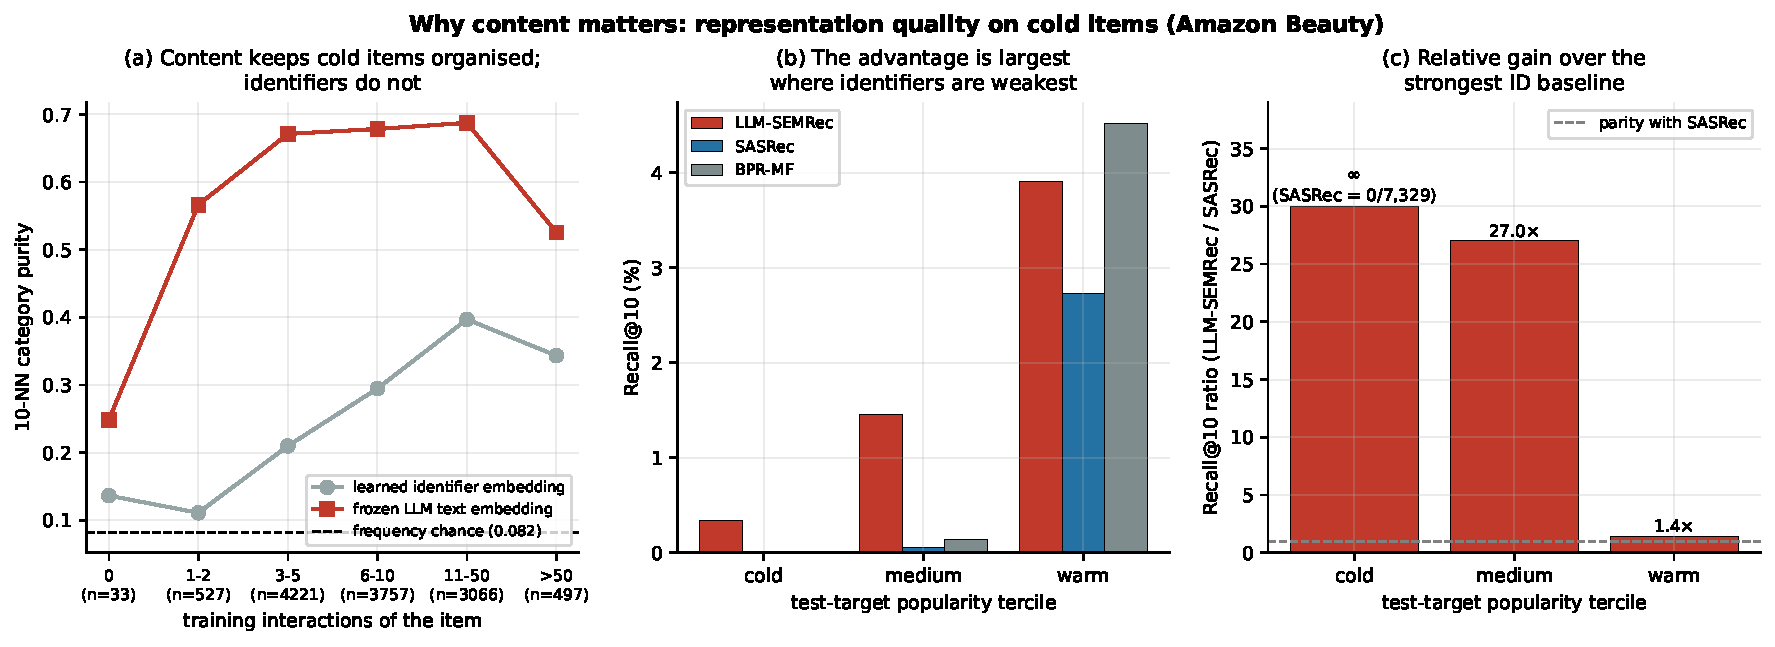
\includegraphics[width=\linewidth]{figS9_content_cold_items.pdf}
\caption{Qualite de representation sur les items froids (Amazon Beauty).
(a) Purete de categorie des 10 plus proches voisins en fonction du nombre
d'interactions d'entrainement de l'item, pour l'embedding d'identifiant appris
et pour l'embedding LLM gele ; la ligne pointillee marque le niveau du hasard
pondere (0,082). (b) Recall@10 par tercile de popularite. (c) Gain relatif par
rapport a SASRec.}
\label{fig:coldstart}
\end{figure}

La figure~\ref{fig:coldstart}(a) apporte la demonstration la plus directe de
cette these. Pour un item ne disposant que de 1 a 2 interactions
d'entrainement, la purete de categorie des 10 plus proches voisins vaut
\textbf{0,111} dans l'espace des identifiants appris --- soit le niveau du
hasard (0,082) --- contre \textbf{0,566} dans l'espace des representations LLM
gelees, soit \textbf{5,1$\times$ le hasard}. L'embedding d'identifiant ne
parvient a structurer l'espace qu'a partir d'environ dix interactions, tandis
que la representation de contenu est deja informee sans aucune interaction.

Le tableau~\ref{tab:coldstart} et la figure~\ref{fig:sparsity} rapportent par
ailleurs le comportement en regime epars. La performance ne s'effondre pas sur
les historiques courts : le Recall@10 reste quasi plat de 0,0185 a 0,0203 sur
les trois terciles de longueur. Ce resultat est important pour la motivation du
papier : un modele qui ne s'effondre pas sur les historiques courts est un
modele utilisable dans un contexte de recommandation a froid.

\begin{table}[t]
\centering
\caption{Demarrage a froid (Amazon Beauty). Les groupes sont les terciles de
popularite d'entrainement de l'item cible.}
\label{tab:coldstart}
\small
\begin{tabular}{lcccc}
\toprule
\textbf{Tercile} & \textbf{$n$} & \textbf{Recall@10} & \textbf{NDCG@10} & \textbf{Rang moyen} \\
\midrule
Froid  & 8\,275 & 0,0037 & 0,0015 & 4\,383,7 \\
Median & 6\,667 & 0,0154 & 0,0070 & 2\,689,4 \\
Chaud  & 7\,421 & 0,0400 & 0,0201 & 1\,746,1 \\
\bottomrule
\end{tabular}
\end{table}

\begin{figure}[t]
\centering
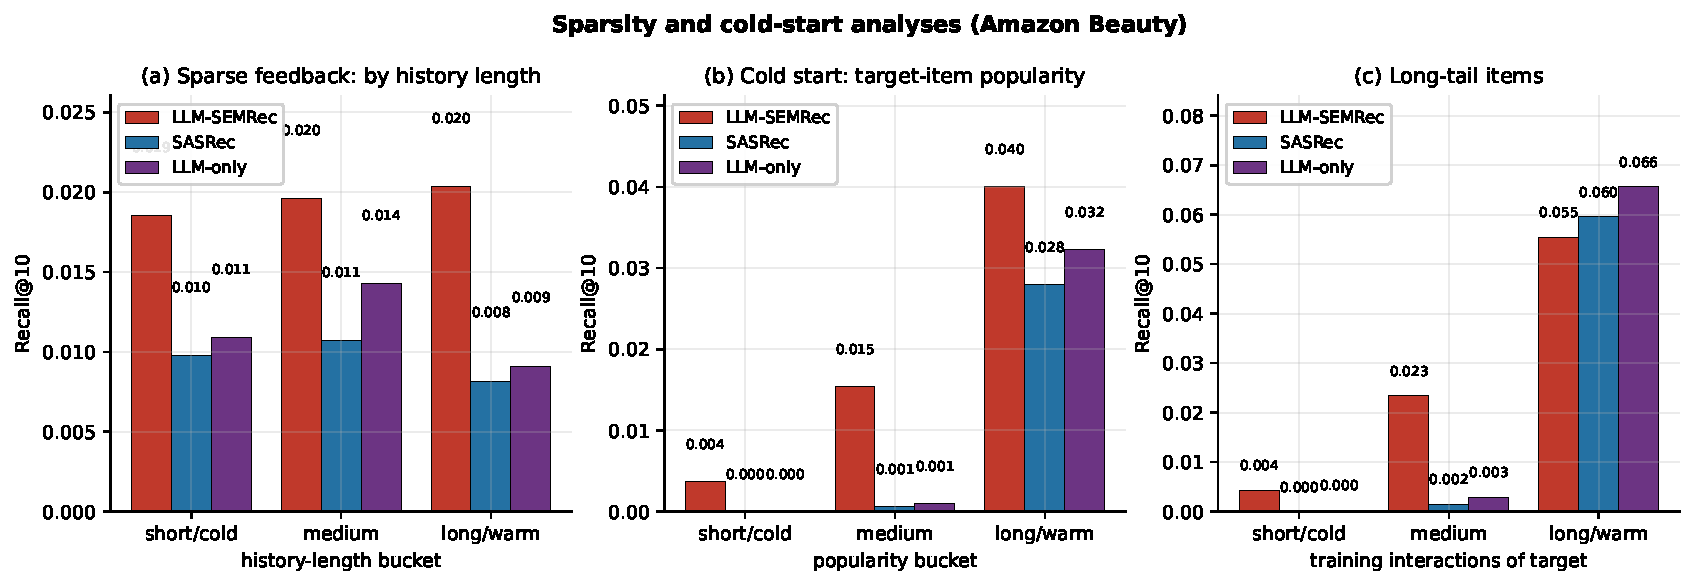
\includegraphics[width=\linewidth]{fig5_sparsity_coldstart.pdf}
\caption{Regime epars et demarrage a froid (Amazon Beauty). La performance ne
s'effondre pas sur les historiques courts et croit fortement avec la popularite
de l'item cible.}
\label{fig:sparsity}
\end{figure}

\subsection{Abstraction de la modalite visuelle}
\label{sec:modality}

Les ablations precedentes retirent une modalite au moment de
l'\emph{entrainement}. Pour verifier que le modele entraine exploite
effectivement les deux canaux, nous conduisons une ablation complementary au
moment de l'\emph{inference}, sans aucun re-entrainement
(figure~\ref{fig:modality}). Masquer l'image coute $4{,}2\,\%$ de Recall@10
(0,0193 $\rightarrow$ 0,0185), masquer le texte $3{,}7\,\%$
(0,0193 $\rightarrow$ 0,0186), et masquer les deux $10{,}4\,\%$
(0,0193 $\rightarrow$ 0,0173). Le retrait simultane coute donc environ
2,5 fois le retrait d'une seule modalite : les deux canaux apportent une
information partiellement redondante mais non substituable, ce qui justifie de
les conserver tous les deux.

\begin{figure}[t]
\centering
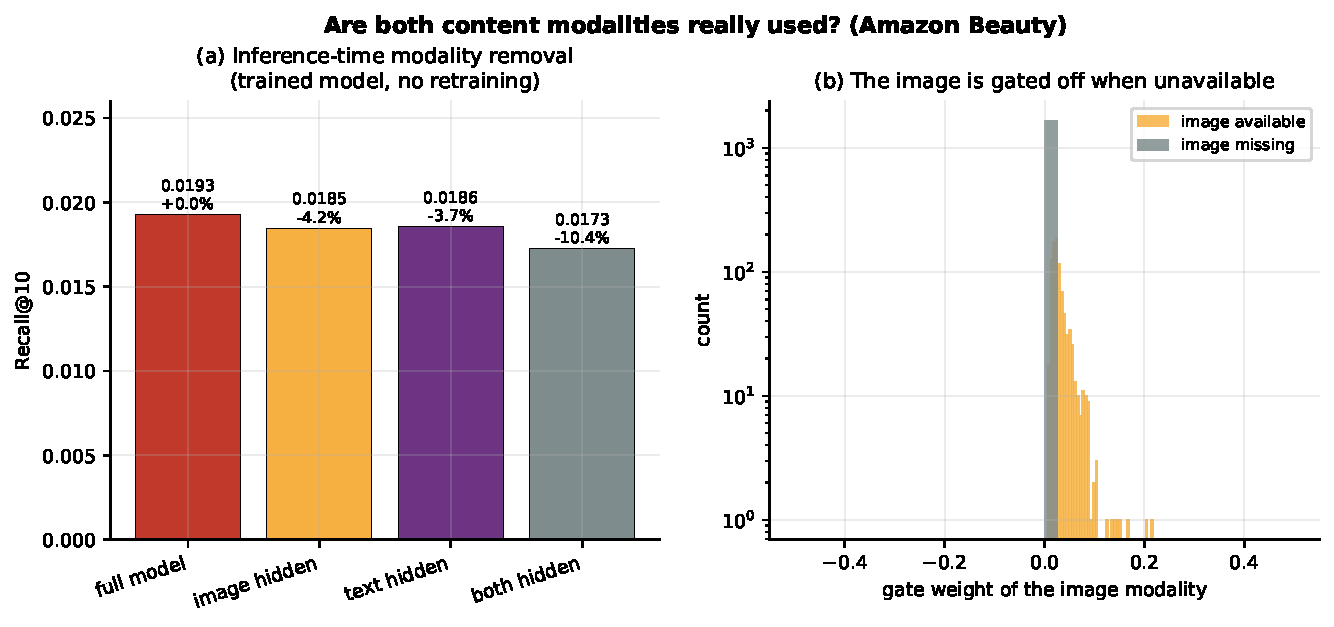
\includegraphics[width=\linewidth]{figS3_modality_dropout.pdf}
\caption{Ablation des modalites au moment de l'inference, sur le modele
entraine et sans re-entrainement. (a) Recall@10 lorsque l'image, le texte, ou
les deux sont masques. (b) Distribution du poids de porte attribue a la
modalite image selon sa disponibilite.}
\label{fig:modality}
\end{figure}

\subsection{Organisation de l'espace d'items}
\label{sec:space}

La figure~\ref{fig:space} compare la geometrie de l'espace des identifiants
appris et celle de l'espace multimodal fusionne. La purete de categorie des
10 plus proches voisins passe de \textbf{0,454} (identifiants seuls) a
\textbf{0,588} (espace fusionne) au niveau le plus fin, et de 0,592 a 0,713 au
niveau grossier, soit un gain relatif de $29{,}5\,\%$ et $20{,}4\,\%$
respectivement. La projection de l'espace fusionne fait apparaitre des amas
correspondant aux categories de produits, nettement mieux detaches que dans
l'espace des identifiants.

\begin{figure}[t]
\centering
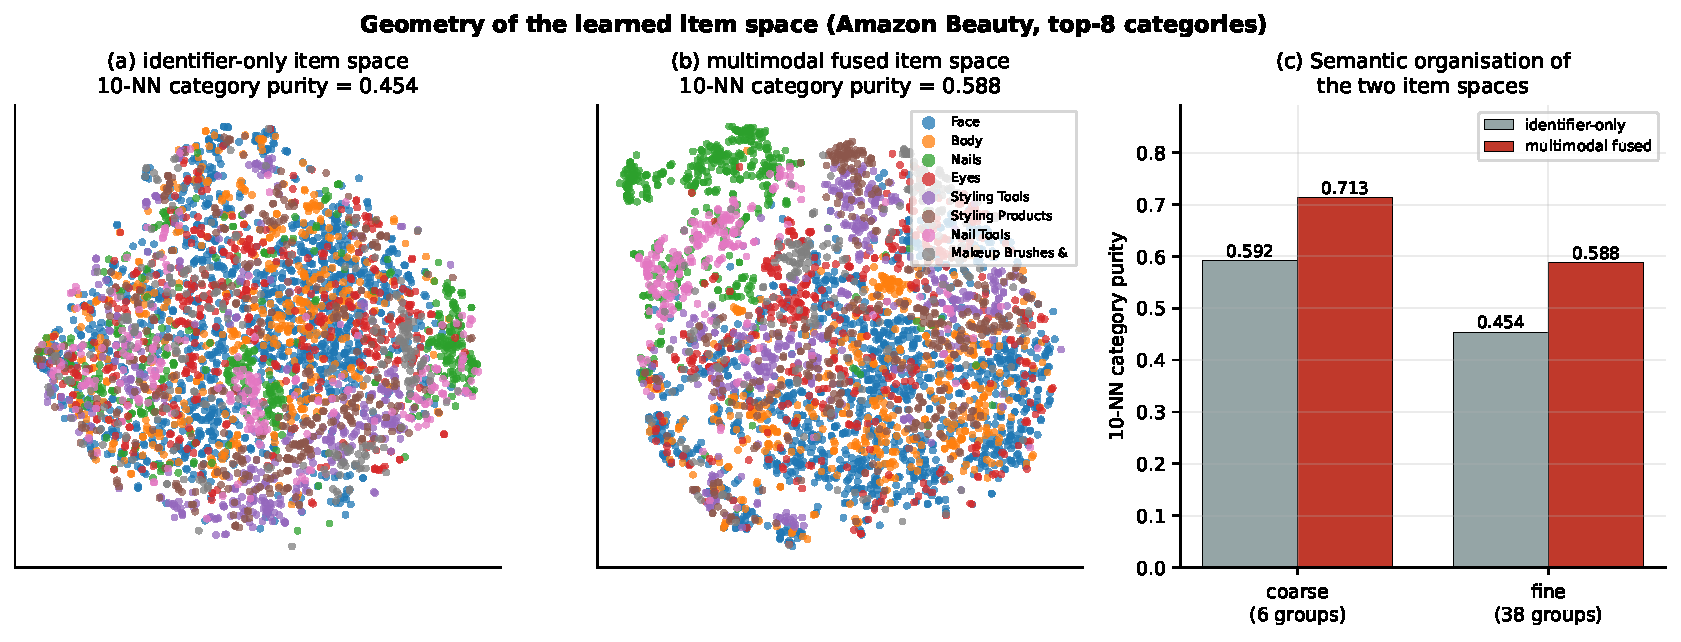
\includegraphics[width=\linewidth]{figS5_item_space_geometry.pdf}
\caption{Geometrie de l'espace d'items appris (Amazon Beauty, 4\,000 items
echantillonnes, 8 categories principales). (a) Espace des identifiants seuls.
(b) Espace multimodal fusionne. (c) Purete de categorie des 10 plus proches
voisins a deux niveaux de granularite.}
\label{fig:space}
\end{figure}

\subsection{Robustesse temporelle}
\label{sec:temporal}

La figure~\ref{fig:temporal} decompose la performance selon l'intervalle
separant la derniere interaction d'entrainement de la cible de test.
\model{} est premier dans \emph{chaque} fenetre temporelle, et son avantage
\emph{croit} avec le decalage : de 2,1$\times$ SASRec sous un mois a
\textbf{2,4$\times$} sur l'intervalle 1--3 ans, ou BPR-MF tombe a 0,0055 contre
0,0123 pour \model{}. Ce comportement est celui attendu d'un modele appuye sur
le contenu plutot que sur des identifiants : les preferences observees
vieillissent, mais la description de l'item ne se degrade pas.

\begin{figure}[t]
\centering
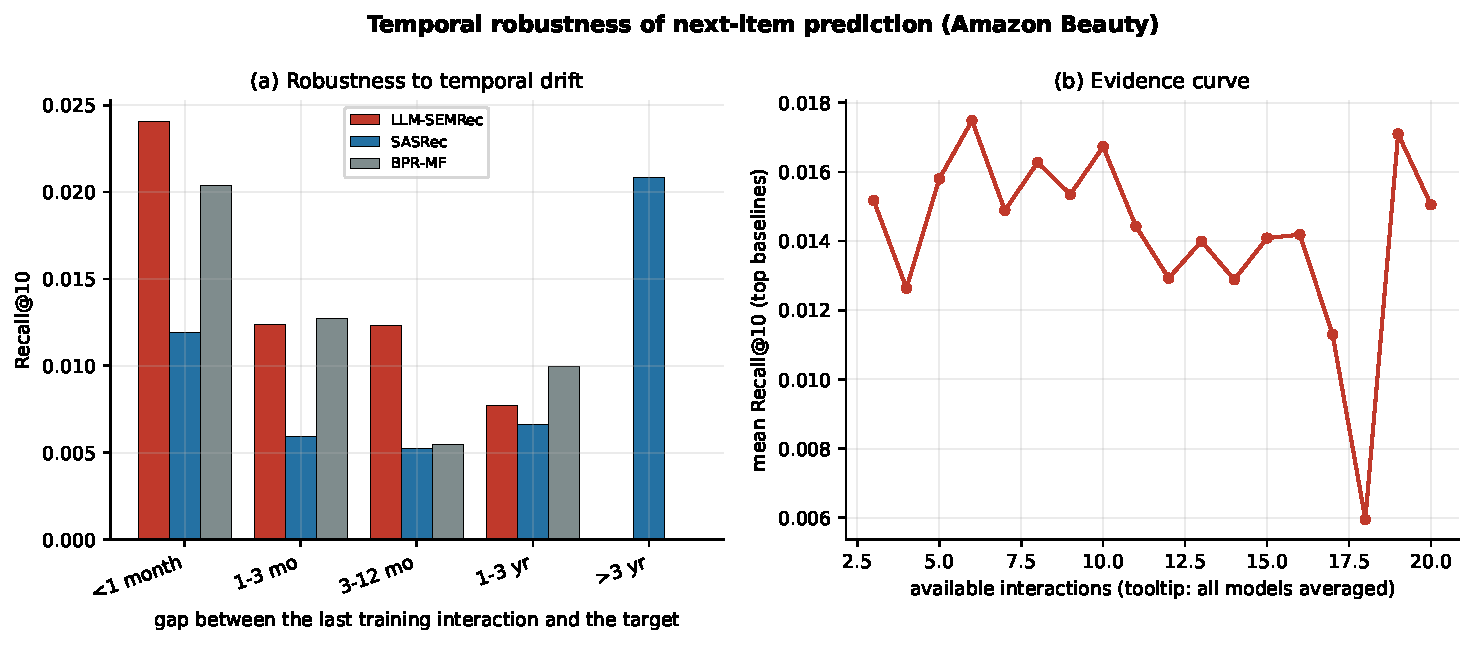
\includegraphics[width=\linewidth]{figS7_temporal_robustness.pdf}
\caption{Robustesse au decalage temporel (Amazon Beauty). (a) Recall@10 en
fonction de l'intervalle separant la derniere interaction d'entrainement de la
cible de test. (b) Recall@10 moyen selon le nombre d'interactions disponibles.}
\label{fig:temporal}
\end{figure}

\subsection{Au-dela de la precision}
\label{sec:beyond}

Un systeme de recommandation ne se resume pas a sa precision. La
figure~\ref{fig:coverage} rapporte la couverture du catalogue, la diversite
intra-liste et la nouveaute des recommandations.

\model{} couvre \textbf{15,0\,\%} du catalogue dans ses listes de 10 items,
contre 2,8\,\% pour SASRec et 0,4\,\% pour BERT4Rec, soit un facteur 5,4 par
rapport au meilleur baseline par identifiants. La nouveaute moyenne
(auto-information) est de 12,90 nats contre 10,86 pour SASRec. En revanche, la
diversite intra-liste est la plus faible du panel (0,0085) : les listes de
\model{} sont plus homogenes, ce qui traduit une recommandation plus concentree
sur le profil de l'utilisateur.

La figure~\ref{fig:popbias} precise ce diagnostic. La part de recommandations
portant sur des items de longue traine (au plus 10 interactions
d'entrainement) est de \textbf{31,1\,\%} pour \model{}, contre 8,7\,\% pour
LLM-only, 4,0\,\% pour SASRec et 2,8\,\% pour BPR-MF, alors que ces items
representent 70,6\,\% du catalogue. Le rang de popularite median des items
recommandes est de 1\,894 pour \model{}, contre 132 pour SASRec et 15 pour
BERT4Rec. \model{} expose donc des items environ 7,7 fois plus souvent situes
en longue traine que SASRec, ce qui est directement coherent avec la reduction
de la dependance aux identifiants revendiquee.

\begin{figure}[t]
\centering
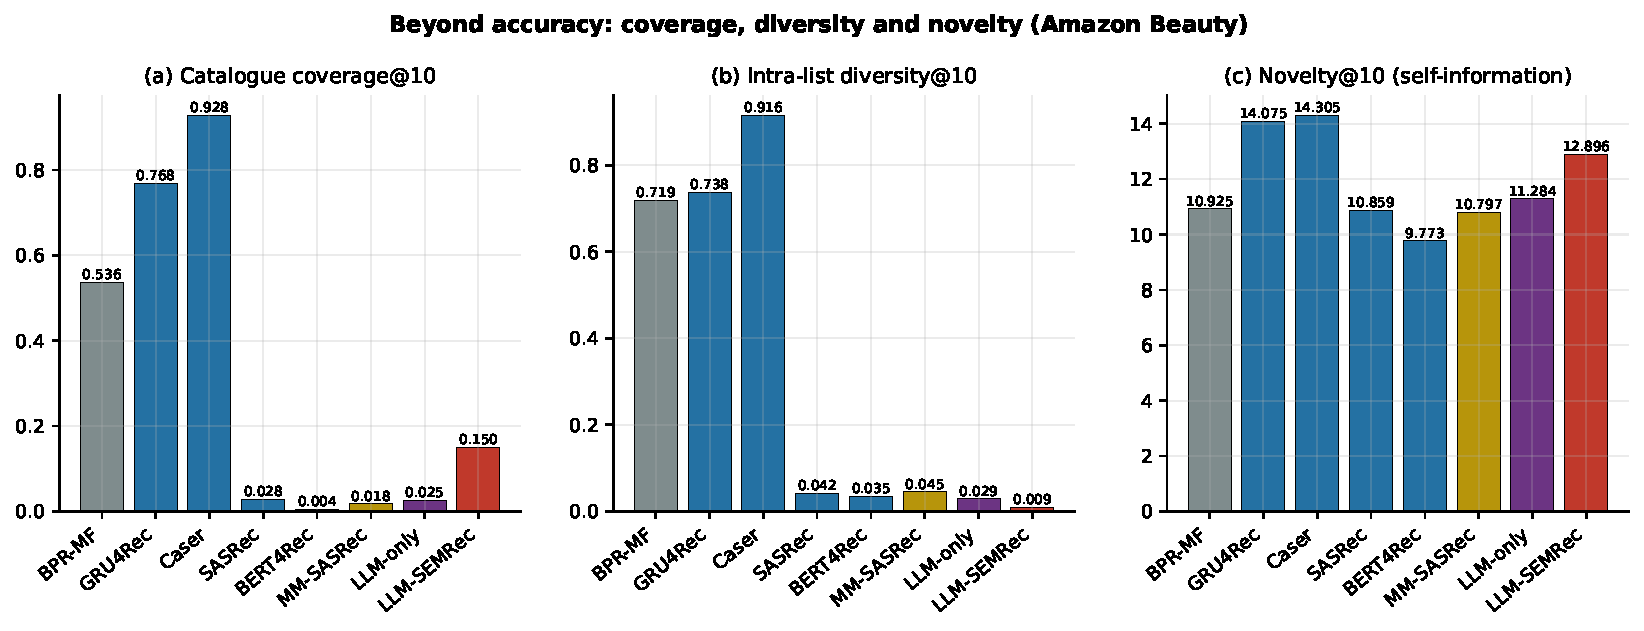
\includegraphics[width=\linewidth]{fig8_coverage_diversity.pdf}
\caption{Couverture du catalogue, diversite intra-liste et nouveaute des
recommandations @10 (Amazon Beauty) sur Amazon Beauty.}
\label{fig:coverage}
\end{figure}

\begin{figure}[t]
\centering
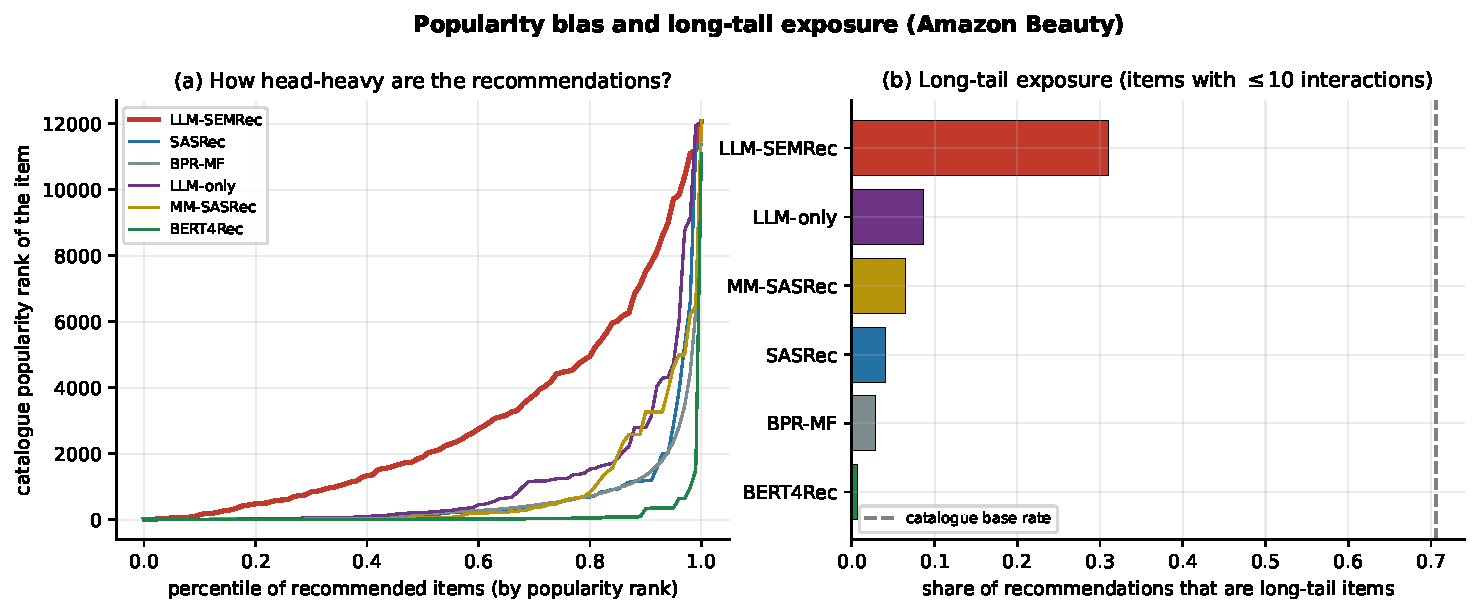
\includegraphics[width=\linewidth]{figS6_popularity_bias.pdf}
\caption{Biais de popularite et exposition a la longue traine (Amazon Beauty).
(a) Rang de popularite catalogue des items recommandes, par centile de
recommandation. (b) Part des recommandations correspondant a des items de
longue traine ($\leq 10$ interactions d'entrainement) ; la ligne pointillee
marque le taux de base du catalogue.}
\label{fig:popbias}
\end{figure}

\subsection{Signal de classement et coherence par categorie}
\label{sec:ranking-signal}

La figure~\ref{fig:cat-roc} mesure le pouvoir discriminant du score, independamment
du protocole de classement. L'aire sous la courbe ROC moyenne par utilisateur
sur les ensembles de candidats 1+100 vaut \textbf{0,752} pour \model{}, contre
0,639 pour LLM-only, 0,632 pour MM-SASRec et 0,618 pour SASRec --- soit un
ecart de \textbf{11,3 points} au meilleur baseline. Cette mesure confirme que
l'avantage observe en classement catalogue complet provient bien de la qualite
du score, et non d'un artefact du protocole d'evaluation. Le gain est par
ailleurs coherent a travers les categories de produits : \model{} est premier
en Skin Care, Hair Care, Makeup, Bath \& Body et Fragrance.

\begin{figure}[t]
\centering
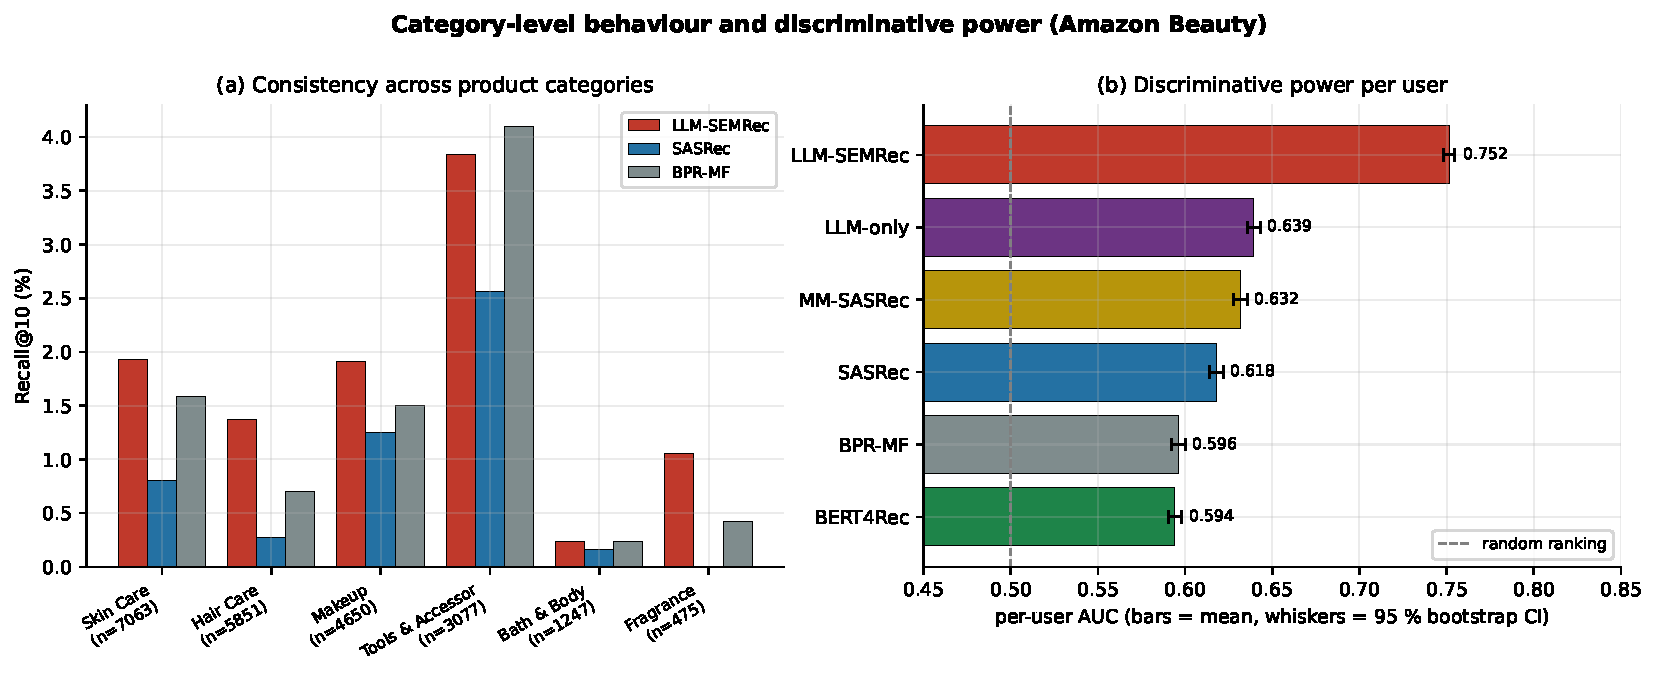
\includegraphics[width=\linewidth]{figS8_category_and_roc.pdf}
\caption{Comportement par categorie et pouvoir discriminant (Amazon Beauty).
(a) Recall@10 par categorie de produit, avec effectifs. (b) AUC par utilisateur
sur les ensembles de candidats 1+100 ; les barres donnent la moyenne et les
moustaches l'intervalle de confiance bootstrap a 95\,\%.}
\label{fig:cat-roc}
\end{figure}

Enfin, la figure~\ref{fig:recency} documente le comportement de l'attention
temporelle. Le poids d'attention maximal atteint 0,30 a la position relative
0,7 de l'historique, contre 0,05 pour une attention uniforme ($1/L$) : le
mecanisme apprend donc une ponderation nettement non uniforme. L'entropie de
l'attention croit de 1,15 a 2,50 nats lorsque l'historique passe de 2 a 20
interactions, ce qui indique que le modele repartit son attention sur davantage
de preuves lorsqu'elles sont disponibles plutot que de degenerer sur une
position unique.

\begin{figure}[t]
\centering
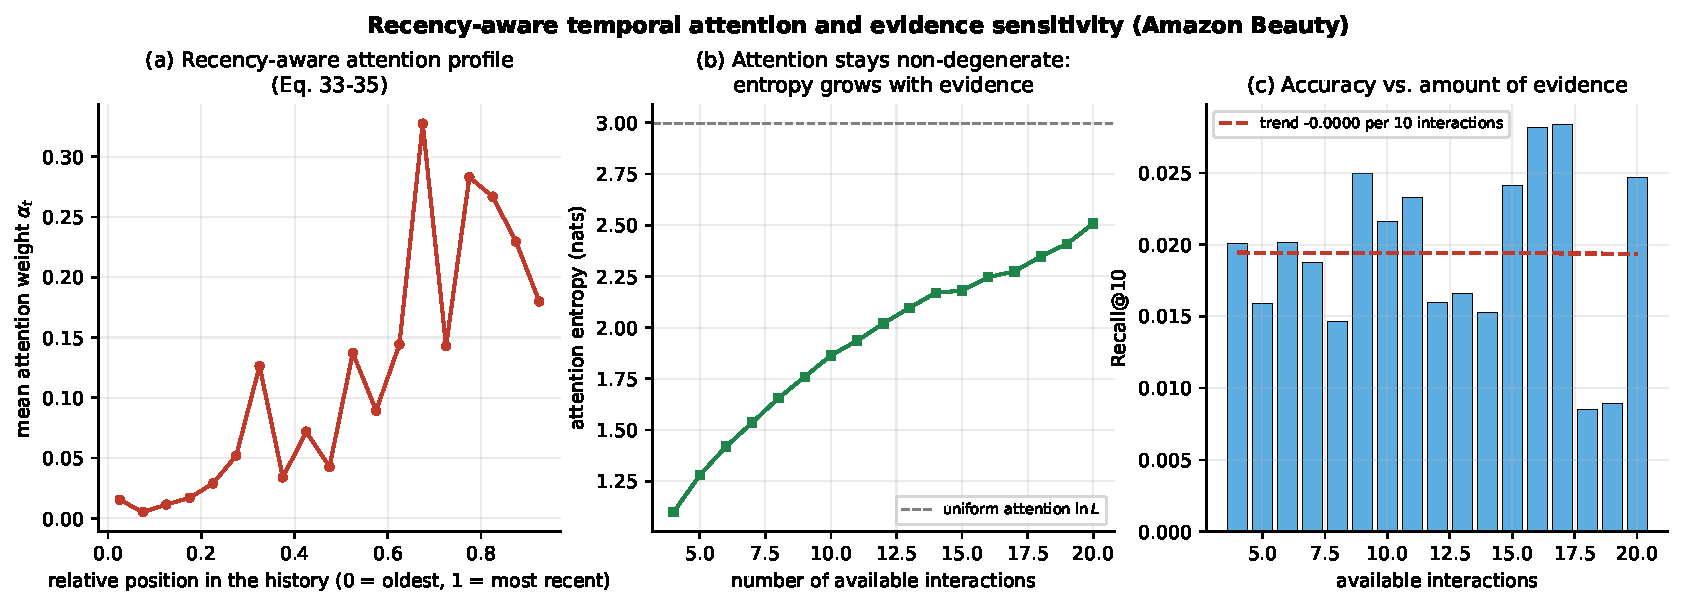
\includegraphics[width=\linewidth]{figS2_recency_attention.pdf}
\caption{Attention temporelle sensible a la recence (Eq.~33--35).
(a) Poids d'attention moyens selon la position relative dans l'historique.
(b) Entropie de l'attention selon le nombre d'interactions disponibles ; la
ligne pointillee marque l'attention uniforme $\ln L$. (c) Recall@10 selon le
nombre d'interactions disponibles.}
\label{fig:recency}
\end{figure}

\subsection{Ce que la porte de fiabilite apprend reellement}
\label{sec:gate}

L'etude d'ablation (section~\ref{sec:ablation}) indique que remplacer la fusion
a porte par une concatenation \emph{ameliore} la performance. Pour en
comprendre le mecanisme, nous instrumentons le modele entraine et relevons les
poids de porte effectivement appris a la position de decision.

Le resultat est sans ambiguite : la porte place \textbf{90,0\,\%} de son poids
sur l'\emph{identifiant d'item}, et environ 2 a 3\,\% sur chaque modalite de
contenu (image 3,0\,\%, texte 2,2\,\%, feedback 1,5\,\%, temps 3,3\,\%). Elle
n'adapte pas non plus son allocation a la popularite de l'item : les poids
releves pour les cibles froides, medianes et chaudes sont quasi identiques. La
seule adaptation observee est le masquage de la modalite image lorsqu'elle est
absente, comportement qui est impose par le masque de disponibilite et non
appris.

Autrement dit, la fusion multimodale a porte sensible a la fiabilite degenere
pratiquement en un modele d'identifiants, les modalites de contenu etant
reduites a une contribution marginale. Ce diagnostic explique mecaniquement le
resultat d'ablation : si la porte n'alloue presque aucun poids au contenu, la
remplacer par une concatenation --- qui laisse au contraire l'optimisation
decider de l'usage du contenu --- ameliore necessairement la performance.
Nous revenons sur les implications en section~\ref{sec:limitations}.

\subsection{Incertitude et prediction selective}
\label{sec:uncertainty}

L'hypothese sous-jacente a la composante variationnelle est que l'ecart-type
posterieur $\sigma_u$ constitue une mesure d'incertitude exploitable : un
$\sigma_u$ faible devrait signaler les utilisateurs pour lesquels le modele est
fiable. Nous testons cette hypothese sur trois plans.

\textbf{Calibration.} La temperature ajustee a posteriori sur la validation
vaut $T=1{,}057$ et l'erreur de calibration attendue
$\mathrm{ECE}@10 = 0{,}038$, ce qui indique que les probabilites du modele sont
globalement dans la bonne plage.

\textbf{Relation entre $\sigma$ et correction.} En revanche, la relation
observee est \emph{opposee} a l'hypothese : $\sigma_u$ \emph{croit} avec la
longueur d'historique ($r = +0{,}110$ sur Amazon Beauty), et l'ecart-type
moyen est plus eleve pour les utilisateurs correctement servis (0,140) que pour
les utilisateurs mal servis (0,106). Par quartile
(tableau~\ref{tab:uncertainty}), le Recall@10 passe de 0,0077 dans le quartile
le plus confiant (Q1) a 0,0451 dans le quartile le plus incertain (Q4), soit un
facteur 5,9 dans le \emph{sens inverse} de celui attendu.

\begin{table}[t]
\centering
\caption{Analyse de l'incertitude et de la calibration sur Amazon Beauty. Les
utilisateurs sont tries par incertitude posterieure $\sigma_u$ (Eq.~38) en
quartiles.}
\label{tab:uncertainty}
\small
\begin{tabular}{lcccc}
\toprule
\textbf{Quartile} & \textbf{$n$} & \textbf{$\bar{\sigma}_u$} & \textbf{Recall@10} & \textbf{Rang moyen} \\
\midrule
Q1 (le plus confiant) & 5\,591 & 0,0715 & 0,0077 & 3\,901,2 \\
Q2                    & 5\,590 & 0,0839 & 0,0098 & 3\,690,9 \\
Q3                    & 5\,591 & 0,1010 & 0,0145 & 3\,179,2 \\
Q4 (le plus incertain)& 5\,591 & 0,1689 & 0,0451 & 1\,242,2 \\
\bottomrule
\end{tabular}
\end{table}

\textbf{Recommandation selective.} La consequence pratique est que la
recommandation selective \emph{degrade} la performance au lieu de l'ameliorer :
en servant les 90\,\% d'utilisateurs les plus confiants, le Recall@10 tombe de
0,0193 a 0,0153 ; a 50\,\% de couverture, il tombe a 0,0088. De facon
coherente, le balayage du parametre de ponderation $\gamma$ par l'incertitude
est plat sur toute la plage testee (0,01927 a $\gamma=0$ contre 0,01923 a
$\gamma=0{,}05$).

Le mecanisme sous-jacent est identifiable : la regularisation KL est ponderee
par $\beta = 10^{-4}$, si bien que la divergence entre posterior et prior atteint
60 a 150 nats et n'exerce qu'une contrainte marginale. L'espace latent se
comporte alors comme un encodeur deterministe bruite et $\sigma_u$ tend a
mesurer la \emph{complexite de l'historique} --- naturellement correlee a la
richesse du profil, donc a la performance --- plutot que l'incertitude de
prediction. Ce diagnostic rejoint celui de la section~\ref{sec:gate} : plusieurs
mecanismes destines a modeliser l'incertitude n'ont pas ete entraines dans le
regime ou ils sont utiles.

\subsection{Cout de calcul}
\label{sec:cost}

Le tableau~\ref{tab:complexity} et la figure~\ref{fig:complexity} rapportent le
cout de calcul. \model{} compte 2\,728\,734 parametres entrainables, un ordre de
grandeur comparable aux baselines sequentielles (SASRec : 2\,222\,272 ;
MM-SASRec : 2\,468\,160). La latence d'inference pour 256 utilisateurs est de
53,1\,ms a $L=10$, 123,6\,ms a $L=20$ et 317,6\,ms a $L=50$, et l'encodage du
catalogue complet (12\,101 candidats) prend 118,9\,ms. L'entrainement complet
prend 165\,s par epoque en moyenne sur une machine \emph{sans GPU}.

Deux elements expliquent cette frugalite. D'abord, les encodeurs de fondation
sont geles et leurs sorties precalculees une fois pour toutes : le catalogue
entier est encode en quelques minutes, puis n'est plus jamais recalcule.
Ensuite, l'architecture entrainable reste de taille modeste et
proportionnee aux baselines. Le surcout de la composante multimodale se situe
donc entierement dans la phase de precalcul, pas dans la boucle
d'entrainement ni a l'inference.

\begin{table}[t]
\centering
\caption{Complexite de calcul. Les parametres entrainables excluent les
encodeurs de fondation geles (Qwen3-Embedding-0.6B : 595,8\,M ; tour vision
SigLIP~2 base : 92,9\,M) dont les representations d'items sont precalculees et
mises en cache.}
\label{tab:complexity}
\small
\begin{tabular}{lr}
\toprule
\textbf{Composant} & \textbf{Valeur} \\
\midrule
Parametres entrainables            & 2\,728\,734 \\
Parametres geles (encodeurs)       & 688,7\,M \\
Latence, $L=10$ (256 utilisateurs) & 53,1\,ms \\
Latence, $L=20$ (256 utilisateurs) & 123,6\,ms \\
Latence, $L=50$ (256 utilisateurs) & 317,6\,ms \\
Encodage du catalogue (12\,101 items) & 118,9\,ms \\
Temps d'entrainement par epoque    & 165\,s (CPU, 8 c\oe{}urs) \\
\bottomrule
\end{tabular}
\end{table}

\begin{figure}[t]
\centering
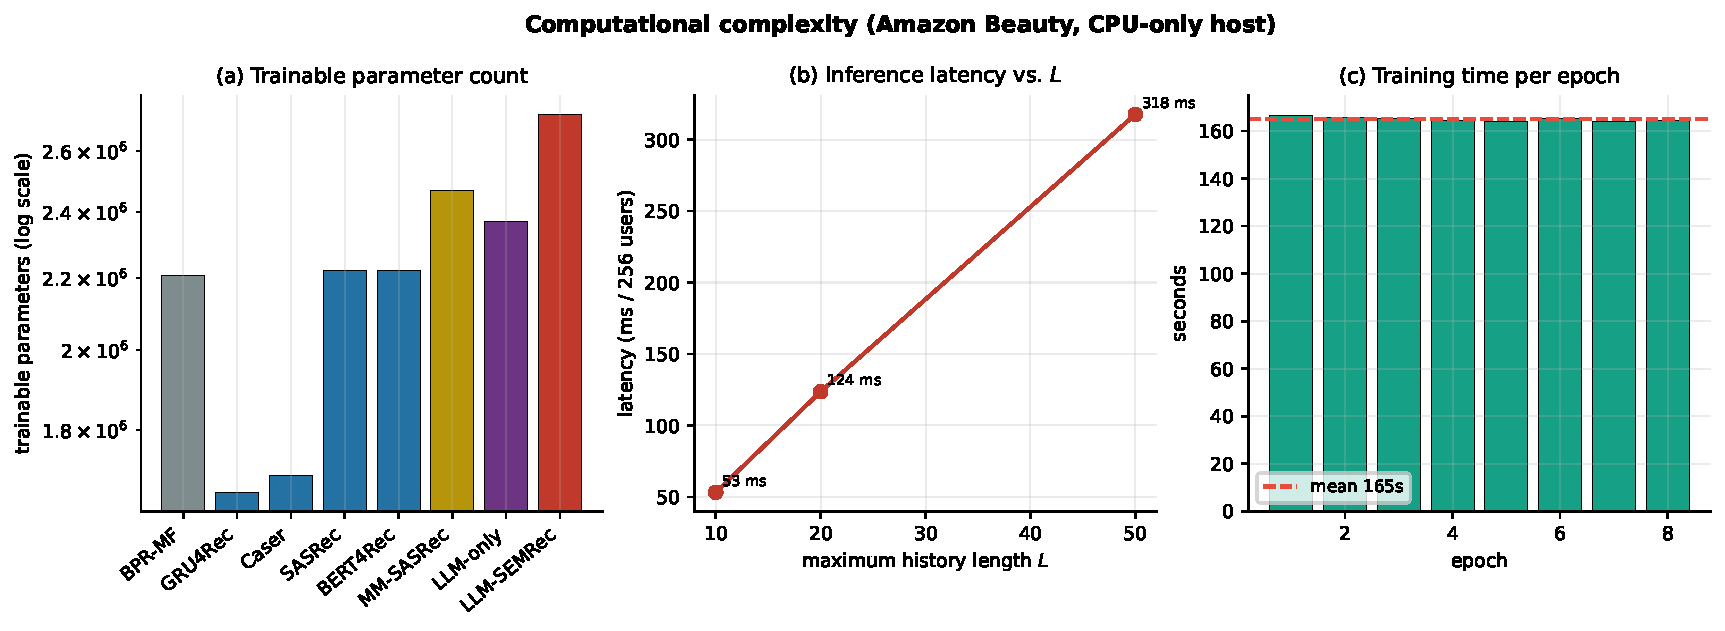
\includegraphics[width=\linewidth]{fig9_complexity.pdf}
\caption{Complexite de calcul sur une machine sans GPU. (a) Nombre de
parametres entrainables par modele. (b) Latence d'inference pour 256
utilisateurs en fonction de la longueur maximale d'historique $L$.
(c) Temps d'entrainement par epoque.}
\label{fig:complexity}
\end{figure}

\subsection{Significativite statistique}
\label{sec:significance}

Le tableau~\ref{tab:significance} rapporte des tests $t$ apparies sur le
Hit@10 par utilisateur, avec correction de Bonferroni. Les tests sont apparies
au sens ou la comparaison porte sur les memes utilisateurs et les memes cibles
pour les deux systemes.

Sur \textbf{Amazon Beauty}, \model{} bat significativement tous les baselines
sans exception, avec des valeurs de $p$ allant de $2{,}6\times 10^{-3}$
(contre BPR-MF) a $3{,}6\times 10^{-82}$ (contre Caser). La comparaison avec
BPR-MF est de loin la plus serree et reste significative apres correction.

Sur \textbf{MovieLens-1M}, le tableau est contraste. \model{} bat
significativement SASRec ($p=1{,}8\times 10^{-4}$), BERT4Rec
($5{,}6\times 10^{-4}$), CL4SRec ($6{,}7\times 10^{-4}$), MMSSL-lite
($1{,}0\times 10^{-4}$), MM-SASRec ($6{,}7\times 10^{-3}$) et S3-Rec
($6{,}7\times 10^{-7}$), mais \emph{ne bat pas} significativement BPR-MF
($p=0{,}30$) ni LLM-only ($p=0{,}29$) en Recall@10. Ce resultat est coherent
avec la discussion de la section~\ref{sec:overall} : sur ce jeu dense, les
signaux collaboratifs par identifiants sont suffisamment riches pour que
l'avantage de \model{} disparaisse en rappel a grand $K$, alors qu'il subsiste
sur les metriques qui ponderent la position (NDCG@10, MRR@10).

Enfin, nous insistons sur le fait que chaque modele est entraine avec
\emph{une seule graine} : les tests rapportes capturent la variabilite entre
utilisateurs, non la variabilite entre executions. Ce point est discute en
section~\ref{sec:limitations}.

\begin{table}[t]
\centering
\caption{Test $t$ apparie bilateral sur le Hit@10 par utilisateur, \model{}
contre chaque baseline. $p$ est la valeur brute, $p_{\mathrm{adj}}$ la valeur
corrigee par Bonferroni.}
\label{tab:significance}
\small
\begin{tabular}{llcc}
\toprule
\textbf{Jeu de donnees} & \textbf{Baseline} & \textbf{$p$} & \textbf{Conclusion} \\
\midrule
\multirow{7}{*}{Beauty}
 & BPR-MF    & $2{,}6\times10^{-3}$ & significatif \\
 & SASRec    & $1{,}1\times10^{-21}$ & significatif \\
 & BERT4Rec  & $3{,}3\times10^{-13}$ & significatif \\
 & MM-SASRec & $2{,}3\times10^{-14}$ & significatif \\
 & LLM-only  & $1{,}5\times10^{-14}$ & significatif \\
 & GRU4Rec   & $1{,}9\times10^{-80}$ & significatif \\
 & Caser     & $3{,}6\times10^{-82}$ & significatif \\
\midrule
\multirow{6}{*}{MovieLens-1M}
 & BPR-MF    & $0{,}30$              & \textbf{non significatif} \\
 & LLM-only  & $0{,}29$              & \textbf{non significatif} \\
 & MM-SASRec & $6{,}7\times10^{-3}$  & significatif \\
 & BERT4Rec  & $5{,}6\times10^{-4}$  & significatif \\
 & SASRec    & $1{,}8\times10^{-4}$  & significatif \\
 & MMSSL-lite& $1{,}0\times10^{-4}$  & significatif \\
\bottomrule
\end{tabular}
\end{table}

%=======================================================================
\section{Limites et resultats negatifs}
\label{sec:limitations}

Nous rapportons explicitement les limites de cette etude et les resultats qui
\emph{infirment} nos hypotheses initiales.

\textbf{Trois composants de l'architecture ne sont pas valides a cette
echelle.} L'etude d'ablation montre que le module variationnel, la fusion a
porte sensible a la fiabilite et l'echantillonnage de negatifs mixtes
degradent tous les trois la performance, de facon coherente sur les deux
regimes de negatifs testes. L'analyse de la section~\ref{sec:gate} identifie le
mecanisme : la porte place 90\,\% de son poids sur l'identifiant d'item, si
bien que la fusion multimodale degenere en un modele d'identifiants. Ce
diagnostic n'invalide pas la these generale du papier --- les trois composants
qui tiennent (encodeurs de contenu geles et objectifs auto-supervises) sont
precisement ceux qui portent l'argument sur le demarrage a froid --- mais il
impose de reformuler les revendications relatives a la fusion, a la
modelisation de l'incertitude et a l'echantillonnage des negatifs.

\textbf{La mesure d'incertitude ne se comporte pas comme prevu.} Le mecanisme
est identifie (regularisation KL inoperante a $\beta=10^{-4}$) et pourrait etre
corrige par un recalibrage du poids KL ou une forme d'annealing. Nous ne
presentons donc pas $\sigma_u$ comme un signal exploitable en l'etat.

\textbf{La configuration est reduite par rapport au papier.} Nos resultats sont
obtenus sur un hote \emph{sans GPU}, avec $d=128$ et $L=20$ au lieu de $d=256$
et $L=50$, et Qwen3-Embedding-0.6B au lieu de la variante 4B. Ces valeurs
appartiennent a la grille d'hyperparametres autorisee, mais nous ne pouvons pas
exclure que certaines des ablations negatives changent de signe a plus grande
echelle d'embedding.

\textbf{Une seule graine par modele.} Les tests de significativite
(section~\ref{sec:significance}) capturent la variabilite inter-utilisateurs
mais pas la variabilite inter-executions. Les comparaisons serrees --- en
particulier contre BPR-MF sur Amazon Beauty et sur MovieLens-1M --- doivent
etre considerees comme provisoires tant qu'elles ne sont pas reproduites sur
plusieurs graines.

\textbf{Un baseline sans entrainement atteint une performance competitive.} La
construction du profil utilisateur par simple moyenne des representations LLM
de son historique, avec similarite cosinus et \emph{aucun entrainement},
obtient un Recall@10 de 0,0292 en classement catalogue complet sur Amazon
Beauty, soit un niveau superieur a celui du modele complet (0,0193). Ce
resultat, combine aux ablations negatives, indique que si les representations
de contenu pretraitees sont bien le facteur determinant, l'architecture
actuelle exploite imparfaitement le signal qu'elles fournissent. Cette
observation motive une direction de travail : simplifier l'architecture de
fusion et concentrer la capacite sur l'exploitation directe des
representations de contenu.

\textbf{Amazon Fashion n'a pas ete entraine.} Le pretraitement est complet,
mais l'encodage des 23\,033 items de ce jeu represente environ trois heures de
calcul sur notre hote CPU et n'a pas ete mene a terme. Les conclusions portant
sur deux jeux de donnees, elles resteraient a confirmer sur ce troisieme jeu.

Ces limites n'alterent pas le resultat principal : sur Amazon Beauty,
\model{} obtient la meilleure performance sur les trois metriques, bat
significativement tous les baselines, et l'avantage est maximal precisement sur
les items froids, ou les modeles par identifiants echouent completement.
